\documentclass[tikz]{standalone}
%\documentclass[tikz]{article}

\usepackage{pgfplots}
\usepackage{ifthen}

\usepackage{amsmath}
\DeclareMathOperator{\sigm}{sigm}
\newcommand{\diff}{\mathop{}\!\mathrm{d}}

\begin{document}

\usetikzlibrary{shapes,arrows,positioning,calc,chains,scopes}

% colors
\definecolor{snowymint}{HTML}{E3F8D1}
\definecolor{wepeep}{HTML}{FAD2D2}
\definecolor{portafino}{HTML}{F5EE9D}
\definecolor{plum}{HTML}{DCACEF}
\definecolor{sail}{HTML}{A3CEEE}
\definecolor{highland}{HTML}{6D885A}

\tikzstyle{signal}=[arrows={-latex},draw=black,line width=1.5pt,rounded corners=4pt]

% RNN
\tikzstyle{block}=[draw=black,line width=1.0pt]
\tikzstyle{cell}=[style=block,draw=highland,fill=snowymint,
    rounded corners]
\tikzstyle{celllayer}=[style=block,draw,fill=portafino,
    inner sep=1pt,outer sep=0,
    minimum width=28pt, minimum height=14pt]
\tikzstyle{pointwise}=[style=block,ellipse,fill=wepeep,
    inner sep=1pt,outer sep=0, minimum size=12pt]

\def\iolen{24pt}
\def\intergape{2pt}

% MLP and CNN
\tikzstyle{netnode}=[circle, inner sep=0pt, text width=22pt, align=center, line width=1.0pt]
\tikzstyle{inputnode}=[netnode, fill=sail,draw=black]
\tikzstyle{hiddennode}=[netnode, fill=snowymint,draw=black]
\tikzstyle{outputnode}=[netnode, fill=plum,draw=black]

% Architecture
\def\layerwidth{90pt}
\def\layerheight{14pt}

\tikzstyle{layer}=[style=block, draw, fill=black!20!white,
    inner sep=1pt,outer sep=0, font=\footnotesize,
    text centered, 
    minimum width=\layerwidth, minimum height=\layerheight]

\tikzstyle{fc}=[style=layer, fill=blue!30!white]
\tikzstyle{conv}=[style=layer, fill=green!30!white]
\tikzstyle{activation}=[style=layer, fill=orange!30!white]
\tikzstyle{pool}=[style=layer, fill=red!30!white]
\tikzstyle{bn}=[style=layer, fill=cyan!30!white]
\tikzstyle{recurrent}=[style=layer, fill=purple!30!white]
\tikzstyle{softmax}=[style=layer, fill=yellow!30!white]
\tikzstyle{point}=[]
\tikzstyle{branch}=[coordinate]

\def\vlayerwidth{30pt}
\def\vlayerheight{3pt}
\def\vblockheight{28pt}

\tikzstyle{vlayer}=[minimum width=\vlayerwidth, minimum height=\vlayerheight]
\tikzstyle{vblock}=[minimum width=\vlayerwidth, minimum height=\vblockheight, text width=1cm, align=center]


% Precision, Recall
\colorlet{fn}{gray!90!green!30!white}
\colorlet{tp}{green!40!white}
\colorlet{fp}{red!40!white}
\colorlet{tn}{gray!90!red!20!white}

% Chain rule, Forward-, Backwardpass
\begin{tikzpicture}[]
    \def\pindist{35pt}
    \def\nodesize{38pt}
    
    \tikzstyle{every pin edge}=[signal]
    \tikzstyle{annot} = [text width=4em, text centered]
    
    \node[hiddennode, text width=\nodesize, minimum size=\nodesize, 
        pin={[pin edge={latex-}, pin distance=\pindist]above left:$x_1$}, 
        pin={[pin edge={latex-}, pin distance=\pindist]below left:$x_2$},
        pin={[pin edge={-latex}, pin distance=\pindist]right:$y_1$}
        ] (N1) at (-100pt,0) {$f(x)$};
    
    \node[hiddennode, text width=\nodesize, minimum size=\nodesize, 
        pin={[pin edge={-latex}, pin distance=\pindist]above left:$\frac{\partial L}{\partial x_1}=\frac{\partial L}{\partial y_1}\frac{\partial y_1}{\partial x_1}$}, 
        pin={[pin edge={-latex}, pin distance=\pindist]below left:$\frac{\partial L}{\partial x_2}=\frac{\partial L}{\partial y_1}\frac{\partial y_1}{\partial x_2}$},
        pin={[pin edge={latex-}, pin distance=\pindist]right:$\frac{\partial L}{\partial y_1}$}
        ] (N2) at (+120pt,0) {$\diff f$};
    
    \node[annot, text width=200pt, align=center, above=40pt of N1] (l1) {Forwardpass};
    \node[annot, text width=200pt, align=center, above=40pt of N2] (l2) {Backwardpass};
    
    \draw[signal, -] (0,-70pt) -- (0,+80pt);
\end{tikzpicture}


% tanh
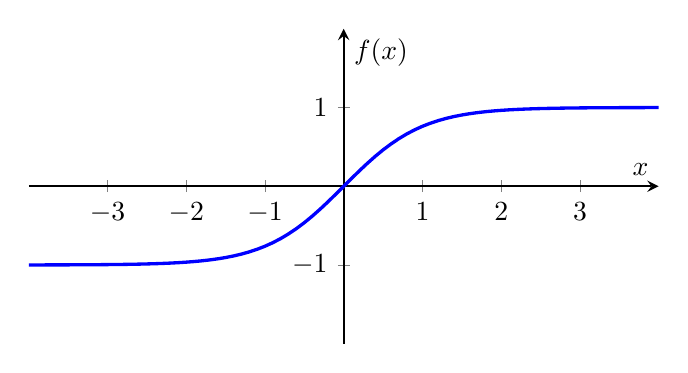
\begin{tikzpicture}[]
\begin{axis}[ 
    %title=$\tanh(x)$,
    axis x line=middle, xmin=-4, xmax=4, xtick={-3,...,3}, xlabel=$x$,
    axis y line=middle, ymin=-2, ymax=2, ytick={-1,...,1}, ylabel=$f(x)$,
    legend pos=north west,
    legend style={empty legend, draw=none},
    scale only axis=true,
    width=8cm, height=4cm,
    thick,
    samples=101] 
    \addplot[blue, very thick] {tanh(x))};
    %\addlegendentry{$\tanh(x)$}
\end{axis}
\end{tikzpicture}

\input{../activation_sigmoid.tex}
\input{../activation_relu.tex}
% Leaky ReLU
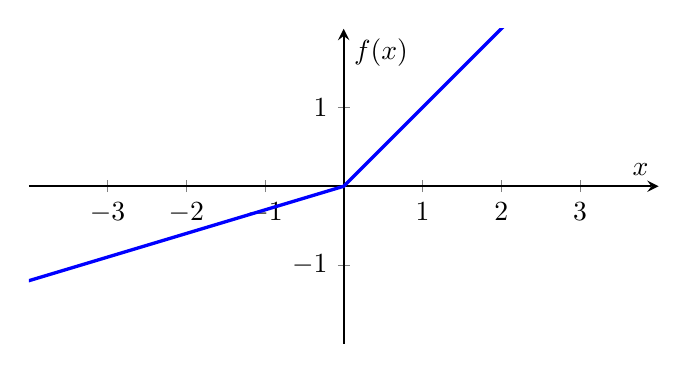
\begin{tikzpicture}[]
\begin{axis}[ 
    %title=$\tanh(x)$,
    axis x line=middle, xmin=-4, xmax=4, xtick={-3,...,3}, xlabel=$x$,
    axis y line=middle, ymin=-2, ymax=2, ytick={-1,...,1}, ylabel=$f(x)$,
    legend pos=north west,
    legend style={empty legend, draw=none},
    scale only axis=true,
    width=8cm, height=4cm,
    thick,
    samples=101] 
    \addplot[blue, very thick] {(\x < 0) * (0.3 * \x) + (\x > 0) * (\x)};
    %\addlegendentry{$\tanh(x)$}
\end{axis}
\end{tikzpicture}


% MLP
\begin{tikzpicture}[]
    \def\nodedist{35pt}
    \def\layerdist{80pt}
    \def\pindist{20pt}
    
    \tikzstyle{every pin edge}=[signal]
    \tikzstyle{annot} = [text width=4em, text centered]
    
    \foreach \y in {1,...,3}
        \node[inputnode, pin={[pin edge={latex-}, pin distance=\pindist]left:Input \y}] 
            (I\y) at (0,-\y*\nodedist) {$x_\y$};  
    
    \foreach \y in {1,...,4}
        \node[hiddennode] 
            (H\y) at ($(\layerdist,-\y*\nodedist) +(0, 0.5*\nodedist)$) {$z_\y$};
    
    \foreach \y in {1,...,1}
        \node[outputnode, pin={[pin edge={-latex}, pin distance=\pindist]right:Output \y}]
            (O\y) at ($(I2) + (2*\layerdist, 0)$) {$y_\y$};
    
    \foreach \dest in {1,...,4}
        \foreach \source in {1,...,3}
            \draw[signal] (I\source) -- (H\dest);
    
    \foreach \dest in {1,...,1}
        \foreach \source in {1,...,4}
            \draw[signal] (H\source) edge (O\dest);
    
    \node[annot, above=4pt of H1] (hl) {Hidden layer};
    \node[annot] at (I1 |- hl) {Input layer};
    \node[annot] at (O1 |- hl) {Output layer};
\end{tikzpicture}

% MLP 2 hidden layers
\begin{tikzpicture}[]
    \def\nodedist{35pt}
    \def\layerdist{80pt}
    \def\pindist{20pt}
    
    \tikzstyle{every pin edge}=[signal]
    \tikzstyle{annot} = [text width=4em, text centered]
    
    \foreach \y in {1,...,3}
        \node[inputnode, pin={[pin edge={latex-}, pin distance=\pindist]left:Input \y}] 
            (I\y) at (0,-\y*\nodedist) {$x_\y$};  

    \foreach \y in {1,...,4}
        \node[hiddennode] 
            (H1\y) at ($(\layerdist,-\y*\nodedist) +(0, 0.5*\nodedist)$) {$z_\y^1$};
    
    \foreach \y in {1,...,4}
        \node[hiddennode] 
            (H2\y) at ($(2*\layerdist,-\y*\nodedist) +(0, 0.5*\nodedist)$) {$z_\y^2$};
    
    \foreach \y in {1,...,2}
        \node[outputnode, pin={[pin edge={-latex}, pin distance=\pindist]right:Output \y}]
            (O\y) at ($(H21) + (\layerdist, -\y*\nodedist)$) {$y_\y$};

    \foreach \dest in {1,...,4}
        \foreach \source in {1,...,3}
            \draw[signal] (I\source) -- (H1\dest);
    
    \foreach \dest in {1,...,4}
        \foreach \source in {1,...,4}
            \draw[signal] (H1\source) -- (H2\dest);
    
    \foreach \dest in {1,...,2}
        \foreach \source in {1,...,4}
            \draw[signal] (H2\source) edge (O\dest);

    \node[annot, above=4pt of H11] (hl) {Hidden layer 1};
    \node[annot, above=4pt of H21] (hl) {Hidden layer 2};
    \node[annot] at (I1 |- hl) {Input layer};
    \node[annot] at (O1 |- hl) {Output layer};
\end{tikzpicture}


\input{../network_layer_fc.tex}
% Convolutional layer
\begin{tikzpicture}[]
    \def\nodedist{30pt}
    \def\layerdist{70pt}
    
    \tikzstyle{every pin edge}=[signal]
    \tikzstyle{annot} = [text width=4em, text centered]

    \foreach \y in {1,...,6}
        \node[hiddennode] 
            (H1\y) at ($(\layerdist,-\y*\nodedist) +(0, 0.5*\nodedist)$) {$z_\y$};
            
    \foreach \y in {1,...,6}
        \node[hiddennode] 
            (H2\y) at ($(2*\layerdist,-\y*\nodedist) +(0, 0.5*\nodedist)$) {$z_\y$};

    \foreach \dest in {1,...,6}
        \draw[signal, red, dashed] (H1\dest) -- (H2\dest);
    
    \foreach \x [count=\xx from 1] in {2,...,6}
        \draw[signal, green, dashed] (H1\xx) -- (H2\x);
    
    \foreach \x [count=\xx from 2] in {1,...,5}
        \draw[signal, blue, dashed] (H1\xx) -- (H2\x);
\end{tikzpicture}


% CNN
\begin{tikzpicture}[]
    \def\nodedist{30pt}
    \def\layerdist{70pt}
    
    \tikzstyle{every pin edge}=[signal]
    \tikzstyle{annot} = [text width=4em, text centered]

    \foreach \y in {1,...,8}
        \node[inputnode] 
            (I\y) at (0,-\y*\nodedist) {$x_\y$};  

    \foreach \y in {1,...,8}
        \node[hiddennode] 
            (H1\y) at (\layerdist,-\y*\nodedist) {$z_\y^{1}$};
            
    \foreach \y in {1,...,8}
        \node[hiddennode] 
            (H2\y) at (2*\layerdist,-\y*\nodedist) {$z_\y^{2}$};
    
    \foreach \y in {1,...,6}
        \node[hiddennode] 
            (H3\y) at (3*\layerdist,-\y*\nodedist-\nodedist) {$z_\y^{3}$};
    
    \foreach \y in {1,...,6}
        \node[outputnode] 
            (O\y) at (4*\layerdist,-\y*\nodedist-\nodedist) {$y_\y$};

    \foreach \dest in {1,...,8}
        \draw[signal, violet] (I\dest) -- (H1\dest);
    \foreach \dest [count=\source from 1] in {2,...,8}
        \draw[signal, teal] (I\source) -- (H1\dest);
    \foreach \dest [count=\source from 2] in {1,...,7}
        \draw[signal, brown] (I\source) -- (H1\dest);

    \foreach \dest in {1,...,8}
        \draw[signal, red,] (H1\dest) -- (H2\dest);
    \foreach \dest [count=\source from 1] in {2,...,8}
        \draw[signal, green] (H1\source) -- (H2\dest);
    \foreach \dest [count=\source from 2] in {1,...,7}
        \draw[signal, blue] (H1\source) -- (H2\dest);

    \foreach \dest in {1,...,6}
        \draw[signal, cyan] (H2\dest) -- (H3\dest);
    \foreach \dest [count=\source from 3] in {1,...,6}
        \draw[signal, orange] (H2\source) -- (H3\dest);
    \foreach \dest [count=\source from 2] in {1,...,6}
        \draw[signal, lime] (H2\source) -- (H3\dest);

    \foreach \dest in {1,...,6}
        \foreach \source in {1,...,6}
            \draw[signal] (H3\source) -- (O\dest);
\end{tikzpicture}

\input{../network_cnn_stide.tex}
\input{../network_cnn_stide2.tex}
% CNN receptive field
\begin{tikzpicture}[]
    \def\nodedist{30pt}
    \def\layerdist{70pt}
    
    \tikzstyle{every pin edge}=[signal]
    \tikzstyle{annot} = [text width=4em, text centered]
    
    \foreach \y in {1,...,14}
        \node[inputnode] 
            (I\y) at (0,-\y*\nodedist) {$x_{\y}$};  
    
    \foreach \y in {1,...,14}
        \node[hiddennode] 
            (H1\y) at (\layerdist,-\y*\nodedist) {$z_{\y}^{1}$};
            
    \foreach \y in {1,...,14}
        \node[hiddennode] 
            (H2\y) at (2*\layerdist,-\y*\nodedist) {$z_{\y}^{2}$};
    
    \foreach \y in {1,...,12}
        \node[hiddennode] 
            (H3\y) at (3*\layerdist,-\y*\nodedist-\nodedist) {$z_{\y}^{3}$};
    
    \foreach \dest in {1,...,14}
        \draw[signal, violet] (I\dest) -- (H1\dest);
    \foreach \dest [count=\source from 1] in {2,...,14}
        \draw[signal, teal] (I\source) -- (H1\dest);
    \foreach \dest [count=\source from 2] in {1,...,13}
        \draw[signal, brown] (I\source) -- (H1\dest);

    \foreach \dest in {1,...,14}
        \draw[signal, red,] (H1\dest) -- (H2\dest);
    \foreach \dest [count=\source from 1] in {2,...,14}
        \draw[signal, green] (H1\source) -- (H2\dest);
    \foreach \dest [count=\source from 2] in {1,...,13}
        \draw[signal, blue] (H1\source) -- (H2\dest);

    \foreach \dest in {1,...,12}
        \draw[signal, cyan] (H2\dest) -- (H3\dest);
    \foreach \dest [count=\source from 3] in {1,...,12}
        \draw[signal, orange] (H2\source) -- (H3\dest);
    \foreach \dest [count=\source from 2] in {1,...,12}
        \draw[signal, lime] (H2\source) -- (H3\dest);
    
    
    \draw [fill=blue, draw=red, fill opacity=0.2, draw opacity=1.0, line width=1.4pt]
        ($(I7) +(-14pt,+21pt)$) -- ($(H39) +(-14pt,+21pt)$) -- ($(H39) +(-14pt,-21pt)$) -- ($(I13) +(-14pt,-21pt)$) -- cycle;
    
\end{tikzpicture}

% unfolding
\begin{tikzpicture}
    \def\nodedist{64pt}
    
    \newcommand{\timestep}[2]{
        \node[block, fill=snowymint, rounded corners, minimum width=40pt, minimum height=24pt] (a#2) at #1 {A};
        \node[inputnode, below=26pt of a#2] (x#2) {$x_#2$};
        \node[outputnode, above=26pt of a#2] (h#2) {$h_#2$};
        \draw[signal] (x#2) -- (a#2);
        \draw[signal] (a#2) -- (h#2);
    }
    
    \timestep{(0, 0)}{t};
    \coordinate (0t) at ($(ht)!0.6!(at)$);
    \draw[signal, -, shorten >=\intergape] (at) -- +(40pt,0pt) |- (0t);
    \draw[signal, latex-, shorten >=\intergape] (at) -- +(-40pt,0pt) |- (0t);
    
    \node[] (e) at ($(at) +(\nodedist,0)$) {\LARGE=};
    
    \timestep{($(e) +(0.7*\nodedist,0)$)}{0};
    \timestep{($(a0) +(\nodedist,0)$)}{1};
    \draw[signal] (a0) -- (a1);
    \timestep{($(a1) +(\nodedist,0)$)}{2};
    \draw[signal] (a1) -- (a2);
    \timestep{($(a2) +(\nodedist,0)$)}{3};
    \draw[signal] (a2) -- (a3);
    
    \node[] at ($(a3) +(0.6*\nodedist,0)$) (ddd) {$\dots$};
    \timestep{($(ddd) +(0.7*\nodedist,0)$)}{t};
    \draw[signal, -] (a3) -- (ddd);
    \draw[signal] (ddd) -- (at);
\end{tikzpicture}


% RNN
\begin{tikzpicture}[thick, node distance=30pt and 30pt, on grid]
    \node[cell, minimum width=200pt, minimum height=110pt, anchor=north west] (b) at (-2pt,0pt) {};
    
    \coordinate (hin) at (0pt,-20pt);
    \draw[signal] (hin) +(-\iolen, 0pt) node[above] {$h_{t-1}$} -- (hin);
    \coordinate (hout) at (200pt,-20pt);
    \draw[signal] (hout) -- +(\iolen,0pt) node[above left] {$h_{t}$};
    \coordinate (h) at (184pt,0pt);
    \draw[signal] (h) -- +(0,\iolen) node[left] {$h_{t}$};
    \coordinate (x) at (14pt,-110pt);
    \draw[signal, -] (x) +(0pt,-\iolen) node[left] {$x_{t}$} -- (x);
    
    \node[celllayer] at (b) (a) {$\tanh$};
    
    \draw[signal, -] (a) |- (hout);
    \draw[signal, -] (hout -| h) +(-10pt,0pt) -| (h);
    \coordinate (hx) at (60pt,-100pt);
    \draw[signal, -] (x) |- (hx);
    \draw[signal, -] (hx) -| (a);
    \draw[signal, -] (hin) +(-10pt,0pt) -| +(50pt,-50pt) |- (hx) +(10pt,0pt);
\end{tikzpicture}

% LSTM
\begin{tikzpicture}[thick, node distance=30pt and 30pt, on grid]
    \node[cell, minimum width=200pt, minimum height=110pt, anchor=north west] (b) at (-2pt,0pt) {};
    
    \coordinate (cin) at (0pt,-20pt);
    \draw[signal] (cin) +(-\iolen, 0pt) node[above] {$c_{t-1}$} -- (cin);
    \coordinate (cout) at (200pt,-20pt);
    \draw[signal] (cout) -- +(\iolen,0pt) node[above left] {$c_{t}$};
    \coordinate (hin) at (0pt,-100pt);
    \draw[signal] (hin) +(-\iolen, 0pt) node[above] {$h_{t-1}$} -- (hin);
    \coordinate (hout) at (200pt,-100pt);
    \draw[signal] (hout) -- +(\iolen,0pt) node[above left] {$h_{t}$};
    \coordinate (h) at (184pt,0pt);
    \draw[signal] (h) -- +(0,\iolen) node[left] {$h_{t}$};
    \coordinate (x) at (14pt,-110pt);
    \draw[signal, -] (x) +(0pt,-\iolen) node[left] {$x_{t}$} -- (x);
    
    \node[celllayer] (f) at (32pt,-80pt) {$\sigm$};
    \node[celllayer, right=34pt of f] (i) {$\sigm$};
    \node[celllayer, right=34pt of i] (c) {$\tanh$};
    \node[celllayer, right=34pt of c] (o) {$\sigm$};
    
    \node[pointwise, above=60pt of f] (fm) {$\times$};
    
    \node[pointwise, above=30pt of c] (cm) {$\times$};
    \node[pointwise, above=30pt of cm] (cmp) {$+$};
    
    \node[pointwise, above right=20pt and 20 pt of o] (om) {$\times$};
    \node[pointwise, above=20pt of om] (omt) {$\tanh$};
    
    \draw[signal] (f) edge node[near start,left] {$f_t$} (fm);
    
    \draw[signal, -] (c) edge node[pos=0.5,left] {$\tilde{c}_t$} (cm); 
    \draw[signal] (cm) to (cmp);
    \draw[signal] (i) |- (cm) node[near start,left] {$i_t$};
    
    \draw[signal] (o) |- (om) node[pos=0.3,left] {$o_t$};
    
    \draw[signal, -] (fm) -- (cmp);
    
    \draw[signal, -] (cmp) -| (omt);
    \draw[signal, -] (omt) -- (om);
    
    \draw[signal] (cin) +(-\iolen, 0) node[above] {$c_{t-1}$} -- +(0,0);
    
    \draw[signal, -] (cin) +(-10pt,0) -- (fm);
    
    \draw[signal] (hin) +(-\iolen, 0) node[above] {$h_{t-1}$} -- +(0,0);
    
    \draw[signal, -] (hin) +(-10pt,0) -| (o);
    \draw[signal, -] (hin) -| (c);
    \draw[signal, -] (hin) -| (i);
    \draw[signal, -] (hin) -| (f);
    
    \draw[signal] (cout) -- +(\iolen,0) node[above left] {$c_{t}$};
    
    \draw[signal, -] (cmp) -- (cout);
    
    \draw[signal] (hout) -- +(\iolen,0) node[above left] {$h_{t}$};
        
    \draw[signal, -] (om) |- (hout);
    
    \draw[signal, -, shorten >=\intergape] (h |- hout) +(-10pt,0) -| (h |- cout);
    \draw[signal, shorten <=\intergape] (h |- cout) -- +(0,\iolen+20pt) node[left] {$h_{t}$};
    
    \draw[signal, -] (x) |- (f |- hin);
\end{tikzpicture}

% GRU
\begin{tikzpicture}[thick, node distance=30pt and 30pt, on grid]
    \node[cell, minimum width=200pt, minimum height=110pt, anchor=north west] (b) at (-2pt,0pt) {};
    
    \coordinate (hin) at (0pt,-20pt);
    \draw[signal] (hin) +(-\iolen, 0pt) node[above] {$h_{t-1}$} -- (hin);
    \coordinate (hout) at (200pt,-20pt);
    \draw[signal] (hout) -- +(\iolen,0pt) node[above left] {$h_{t}$};
    \coordinate (h) at (184pt,0pt);
    \draw[signal] (h) -- +(0,\iolen) node[left] {$h_{t}$};
    \coordinate (x) at (14pt,-110pt);
    \draw[signal, -] (x) +(0pt,-\iolen) node[left] {$x_{t}$} -- (x);
    
    \node[celllayer] (r) at (68pt,-80pt) {$\sigm$};
    \node[celllayer, right=58pt of r] (z) {$\sigm$};
    \node[celllayer, right=34pt of z] (ht) {$\tanh$};
    
    \node[pointwise, above=30pt of ht] (htm) {$\times$};
    \draw[signal] (ht) edge node[pos=0.5,left] {$\tilde{h}_t$} (htm);
    \node[pointwise, above=30pt of htm] (htmp) {$+$};
    \draw[signal] (htm) -- (htmp);
    \draw[signal, -] (htmp) -- (hout);
    
    \node[pointwise, above left=30pt and 30pt of z] (z1) {$-1$};
    \draw[signal] (z) |- (z1) node[pos=0.2,left] {$z_t$};
    \node[pointwise, above=30pt of z1] (z1m) {$\times$};
    \draw[signal] (z1) -- (z1m);
    \draw[signal, -] (z1m) -- (htmp);
    \draw[signal] (z) |- (htm);
    \draw[signal, -] (hout -| h) +(-10pt,0pt) -| (h);
    
    \draw[signal, -] (hin) +(-10pt,0pt) -- (z1m);
    
    \node[pointwise, above left=30pt and 30pt of r] (rm) {$\times$};
    \draw[signal] (r) |- (rm) node[pos=0.2,left] {$r_t$};
    \draw[signal] (hin -| rm) +(-10pt,0pt) -| (rm);
    
    \coordinate (hx) at (60pt,-94pt);
    \draw[signal, -] (x) |- (hx);
    \draw[signal, -] (hin) +(-10pt,0pt) -| (x |- r) |- (hx) +(10pt,0pt);
    \draw[signal, -] (hx) -| (r);
    \draw[signal, -] (hx) -| (z);
    
    \coordinate (rx) at (60pt,-102pt);
    \draw[signal, -] (x) |- (rx);
    \draw[signal, -] (rx) -| (ht);
    
    \draw[signal, -, shorten >=\intergape] (rm) |- (rm |- hx);
    \draw[signal, -, shorten <=\intergape] (rm |- hx) |- (z |- rx);
\end{tikzpicture}


% RNN legend
\begin{tikzpicture}
	\def\labeldist{30pt}
	\def\nodedist{60pt}

	\node[celllayer, minimum width=40pt] (l) at (0pt,0pt) {};
	\node[align=center] at ($(l) +(0pt,-\labeldist)$) {Network\\Layer}; % trainable
	\node[pointwise] (p) at ($(l) +(\nodedist, 0pt)$) {};
	\node[align=center] at ($(p) +(0pt,-\labeldist)$) {Pointwise\\Operation};
	\coordinate (v) at ($(p) +(\nodedist, 0pt)$);
	\draw[signal] (v) +(-20pt,0pt) -- +(20pt, 0pt);
	\node[align=center] at ($(v) +(0pt,-\labeldist)$) {Vector\\Transfer};
	\coordinate (m) at ($(v) +(\nodedist, 0pt)$);
	\draw[signal] (m) +(-10pt,10pt) |- +(10pt, 0pt);
	\draw[signal] (m) +(-10pt,-10pt) |- +(10pt, 0pt);
	\node[align=center] at ($(m) +(0pt,-\labeldist)$) {Concatenate};
	\coordinate (c) at ($(m) +(\nodedist, 0pt)$);
	\draw[signal] (c) +(-10pt,0pt) -| +(10pt, 12pt);
	\draw[signal] (c) +(-10pt,0pt) -| +(10pt, -12pt);
	\node[align=center] at ($(c) +(0pt,-\labeldist)$) {Copy};
\end{tikzpicture}

% RNN legend, horizontal
\begin{tikzpicture}
    \def\nodedist{170pt}

    \node[celllayer, minimum width=40pt] (l) at (0pt,0pt) {};
    \node[anchor=west] at ($(l) +(30pt, 0pt)$) {Network Layer}; % trainable
    \node[pointwise] (p) at ($(l) +(\nodedist, 0pt)$) {};
    \node[anchor=west] at ($(p) +(16pt, 0pt)$) {Pointwise Operation};
    \coordinate (v) at ($(p) +(\nodedist, 0pt)$);
    \draw[signal] (v) +(-20pt,0pt) -- +(20pt, 0pt);
    \node[anchor=west] at ($(v) +(30pt, 0pt)$) {Vector Transfer};
    \coordinate (m) at ($(v) +(\nodedist, 0pt)$);
    \draw[signal] (m) +(-10pt,10pt) |- +(10pt, 0pt);
    \draw[signal] (m) +(-10pt,-10pt) |- +(10pt, 0pt);
    \node[anchor=west] at ($(m) +(20pt, 0pt)$) {Concatenate};
    \coordinate (c) at ($(m) +(\nodedist, 0pt)$);
    \draw[signal] (c) +(-10pt,0pt) -| +(10pt, 12pt);
    \draw[signal] (c) +(-10pt,0pt) -| +(10pt, -12pt);
    \node[anchor=west] at ($(c) +(20pt, 0pt)$) {Copy};
\end{tikzpicture}


\input{../pooling_max.tex}
% average pooling, kernel (2,2), stride (2,2)
\begin{tikzpicture}
    \coordinate (p) at (0,0);
    \draw[shift={(p)}, fill=red!20!white] (0,0) rectangle (2,-2);
    \draw[shift={(p)}, fill=yellow!20!white] (2,0) rectangle (4,-2);
    \draw[shift={(p)}, fill=blue!20!white] (0,-2) rectangle (2,-4);
    \draw[shift={(p)}, fill=green!20!white] (2,-2) rectangle (4,-4);
    \draw[
        ultra thick,
        step=1, 
        color=black,
        draw=black,
        fill=black!20!white,
        shift={(p)}
    ] (0,0) grid (4,-4)
    foreach[count=~] \l in {73, 74, 17, 49, 10, 29, 41, 20, 4, 23, 39, 4, 50, 80, 56, 57} {
        ({0.5+mod(~-1,4}, {-0.5-div(~-1,4}) node {\Large \l}
    };
    
    \draw[signal] (4.5,-2) -> (5.5, -2);
    
    \coordinate (p) at (6,-1);
    \draw[shift={(p)}, fill=red!20!white] (0,0) rectangle (1,-1);
    \draw[shift={(p)}, fill=yellow!20!white] (1,0) rectangle (2,-1);
    \draw[shift={(p)}, fill=blue!20!white] (0,-1) rectangle (1,-2);
    \draw[shift={(p)}, fill=green!20!white] (1,-1) rectangle (2,-2);
    \draw[
        ultra thick,
        step=1, 
        color=black,
        draw=black,
        fill=black!20!white,
        shift={(p)}
    ] (0,0) grid (2,-2)
    foreach[count=~] \l in {46, 32, 39, 39} {
        ({0.5+mod(~-1,2}, {-0.5-div(~-1,2}) node {\Large \l}
    };
\end{tikzpicture}

% pooling, kernel (3,3), stride (2,2)
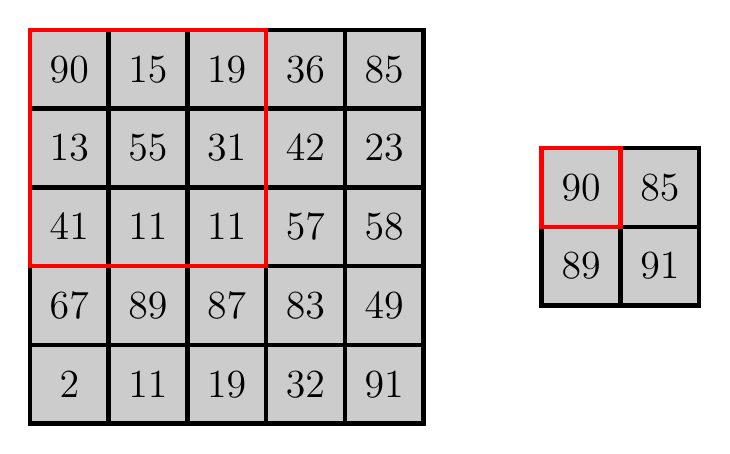
\begin{tikzpicture}
    \coordinate (p) at (0,0);
    \draw[
        ultra thick,
        step=1, 
        color=black,
        draw=black,
        fill=black!20!white,
        shift={(p)}
    ] (0,0) grid (5,-5) rectangle (0,0)
    foreach[count=~] \l in {90, 15, 19, 36, 85, 13, 55, 31, 42, 23, 41, 11, 11, 57, 58, 67, 89, 87, 83, 49,  2, 11, 19, 32, 91} {
        ({0.5+mod(~-1,5}, {-0.5-div(~-1,5}) node {\Large \l}
    };
    \draw[shift={(p)}, draw=red, ultra thick] (0,0) rectangle (3,-3);
    
    \coordinate (p) at (6.5,-1.5);
    \draw[
        ultra thick,
        step=1, 
        color=black,
        draw=black,
        fill=black!20!white,
        shift={(p)}
    ] (0,0) grid (2,-2) rectangle (0,0)
    foreach[count=~] \l in {90, 85, 89, 91} {
        ({0.5+mod(~-1,2}, {-0.5-div(~-1,2}) node {\Large \l}
    };
    \draw[shift={(p)}, draw=red, ultra thick] (0,0) rectangle (1,-1);
    % max     {90, 85, 89, 91}
    % average {32, 40, 38, 54}
\end{tikzpicture}


\input{../pooling_both.tex}

% Residual Block

\begin{tikzpicture}[start chain=going below, node distance=12pt,
        point/.append style={on chain, join=by {signal}},
        layer/.append style={on chain, join=by {signal}},
        branch/.append style={on chain, join=by {signal, -}},
    ]
    \def\branchy{30pt}
    
    \node[point] {Input};
    \node[branch] (input) {};
    \node[conv, xshift=\layerwidth/2+16pt, yshift=-\branchy] {Conv};
    \node[bn] {BatchNorm};
    \node[activation] {ReLU};
    \node[conv] {Conv};
    \node[bn] {BatchNorm};
    \node[layer, xshift=-\layerwidth/2-16pt, yshift=-\branchy] (add) {Addition};
    \node[activation] {ReLU};
    \node[point] {Output};
    \draw[signal] (input) -- (add);
\end{tikzpicture}

% Residual Block 2

\begin{tikzpicture}[start chain=going below, node distance=12pt,
        point/.append style={on chain, join=by {signal}},
        layer/.append style={on chain, join=by {signal}},
        branch/.append style={on chain, join=by {signal, -}},
    ]
    \def\branchy{30pt}
    
    \node[point] {Input};
    \node[branch] (input) {};
    \node[bn, xshift=\layerwidth/2+16pt, yshift=-\branchy] {BatchNorm};
    \node[activation] {ReLU};
    \node[conv] {Conv};
    \node[bn] {BatchNorm};
    \node[activation] {ReLU};
    \node[conv] {Conv};
    \node[layer, xshift=-\layerwidth/2-16pt, yshift=-\branchy] (add) {Addition};
    \node[point] {Output};
    \draw[signal] (input) -- (add);
\end{tikzpicture}

% Inception Block

\begin{tikzpicture}[start chain=main going below, node distance=12pt,
        point/.append style={on chain, join=by {signal}},
        layer/.append style={on chain, join=by {signal}},
        branch/.append style={on chain, join=by {signal, -}},
    ]
    \def\branchy{70pt}
    
    \node[point] {Input};
    \node[branch] {};
    {[start branch=b1 going below]
        \node[conv, xshift=-\layerwidth*1.5-24pt, yshift=-\branchy-26pt] {Conv 1x1};
        \node[activation] {ReLU};
    }
    {[start branch=b2 going below]
        \node[conv, xshift=-\layerwidth*0.5-8pt, yshift=-\branchy] {Conv 1x1};
        \node[activation] {ReLU};
        \node[conv] {Conv 3x3};
        \node[activation] {ReLU};
    }
    {[start branch=b3 going below]
        \node[conv, xshift=\layerwidth*0.5+8pt, yshift=-\branchy] {Conv 1x1};
        \node[activation] {ReLU};
        \node[conv] (foo) {Conv 5x5};
        \node[activation] {ReLU};
    }
    \node[pool, xshift=\layerwidth*1.5+24pt, yshift=-\branchy-13pt] {MaxPool 3x3};
    \node[conv] {Conv 1x1};
    \node[activation] {ReLU};
    \node[layer, xshift=-\layerwidth*1.5-24pt, yshift=-\branchy,
        join=with main/b1-end by signal,
        join=with main/b2-end by signal, 
        join=with main/b3-end by signal] {Concatenation};
    \node[point] {Output};
\end{tikzpicture}

% Dense Block

\begin{tikzpicture}[thick, node distance=\vlayerheight, on grid]
    
    \coordinate (labelcoord) at (\vlayerwidth/2-2pt, 6pt);
    
    \coordinate (n0) at (0,0);
    \coordinate (n1) at ($(n0) +(0pt, -4pt)$);
    \node[anchor=north west] at ($(n1) +(-2pt, 6pt)$) {\tiny wxhxc};
    
    \foreach \y in {1,...,8} {
        \begin{scope} [start chain=going below, every node/.style={on chain}]
            \node[bn, vlayer] (n3) at ($(n1) +(0.8*\vlayerwidth, -20pt)$) {};
            \node[activation, vlayer] {};
            \node[conv, vlayer] (n4) {};
            \node[bn, vlayer] {};
            \node[activation, vlayer] {};
            \node[conv, vlayer] (n2) {};
        \end{scope}
        
        \node[anchor=north west] at ($(n4) +(labelcoord)$) {\tiny 1,1,4k};
        \node[anchor=north west] at ($(n2) +(labelcoord)$) {\tiny 3,1,k};
        \draw[signal] (n1) |- +(8pt, -8pt) -| (n3);
        \coordinate (n1) at ($(n2) +(-0.8*\vlayerwidth, -16pt)$);
        \draw[signal, -] (n2) |- +(-8pt, -8pt) -| (n1);
        \node[anchor=north west] at ($(n1) +(-2pt, 6pt)$) {\tiny wxhx(c+\y k)};
    }
    
    \draw[signal] (n0) -- ($(n1) +(0pt, -12pt)$);
    
\end{tikzpicture}


% AlexNet
\begin{tikzpicture}[start chain=going below, node distance=12pt,
        point/.append style={on chain, join=by {signal}},
        layer/.append style={on chain, join=by {signal}},
    ]
    \node[point] {Input Image};
    \node[conv] {Conv 11x11/4, 96};
    \node[activation] {ReLU};
    \node[pool] {MaxPool 2x2/2};
    % local contrast norm
    \node[conv] {Conv 5x5, 256};
    \node[activation] {ReLU};
    % local contrast norm
    \node[pool] {MaxPool 2x2/2};
    \node[conv] {Conv 3x3, 384};
    \node[activation] {ReLU};
    \node[conv] {Conv 3x3, 384};
    \node[activation] {ReLU};
    \node[conv] {Conv 3x3, 256};
    \node[activation] {ReLU};
    \node[pool] {MaxPool 2x2/2};
    \node[layer] {Flatten};
    \node[fc] {FC 4096};
    \node[activation] {ReLU};
    \node[layer] {Dropout};
    \node[fc] {FC 4096};
    \node[activation] {ReLU};
    \node[layer] {Dropout};
    \node[fc] {FC 1000};
    \node[softmax] {Softmax};
    \node[point] {Classification Output};
\end{tikzpicture}

% VGG16
\begin{tikzpicture}[start chain=going below, node distance=12pt,
        point/.append style={on chain, join=by {signal}},
        layer/.append style={on chain, join=by {signal}},
    ]
    \node[point] {Input Image};
    \node[conv] {Conv 3x3, 64};
    \node[activation] {ReLU};
    \node[conv] {Conv 3x3, 64};
    \node[activation] {ReLU};
    \node[pool] {MaxPool 2x2/2};
    \node[conv] {Conv 3x3, 64};
    \node[activation] {ReLU};
    \node[conv] {Conv 3x3, 64};
    \node[activation] {ReLU};
    \node[pool] {MaxPool 2x2/2};
    \node[conv] {Conv 3x3, 256};
    \node[activation] {ReLU};
    \node[conv] {Conv 3x3, 256};
    \node[activation] {ReLU};
    \node[conv] {Conv 3x3, 256};
    \node[activation] {ReLU};
    \node[pool] {MaxPool 2x2/2};
    \node[conv] {Conv 3x3, 512};
    \node[activation] {ReLU};
    \node[conv] {Conv 3x3, 512};
    \node[activation] {ReLU};
    \node[conv] {Conv 3x3, 512};
    \node[activation] {ReLU};
    \node[pool] {MaxPool 2x2/2};
    \node[conv] {Conv 3x3, 512};
    \node[activation] {ReLU};
    \node[conv] {Conv 3x3, 512};
    \node[activation] {ReLU};
    \node[conv] {Conv 3x3, 512};
    \node[activation] {ReLU};
    \node[pool] {MaxPool 2x2/2};
    \node[layer] {Flatten};
    \node[fc] {FC 4096};
    \node[activation] {ReLU};
    \node[layer] {Dropout};
    \node[fc] {FC 4096};
    \node[activation] {ReLU};
    \node[layer] {Dropout};
    \node[fc] {FC 1000};
    \node[softmax] {Softmax};
    \node[point] {Classification Output};
\end{tikzpicture}

% SSD

\begin{tikzpicture}
    
    \def\d{10pt}
    \def\nd{12pt}
    
    \coordinate (shapecoord) at (\layerwidth/2+4pt, -\d+6pt);
    
    \tikzstyle{stack}=[start chain=going below, 
            node distance=\nd, 
            every node/.style={on chain}, 
            layer/.append style={join=by {signal}},
            point/.append style={join=by {signal}},
        ]
    
    \begin{scope} [stack]
        \node[point] (n0) {Input Image};
        \node[conv] {Conv 3x3, 64};  % conv_1_1
        \node[activation] {ReLU};
        \node[conv] {Conv 3x3, 64};  % conv_1_2
        \node[activation] {ReLU};
        \node[pool] {MaxPool 2x2/2};
        \node[conv] {Conv 3x3, 128}; % conv_2_1
        \node[activation] {ReLU};
        \node[conv] {Conv 3x3, 128}; % conv_2_2
        \node[activation] {ReLU};
        \node[pool] {MaxPool 2x2/2};
        \node[conv] {Conv 3x3, 256}; % conv_3_1
        \node[activation] {ReLU};
        \node[conv] {Conv 3x3, 256}; % conv_3_2
        \node[activation] {ReLU};
        \node[conv] {Conv 3x3, 256}; % conv_3_3
        \node[activation] {ReLU};
        \node[pool] {MaxPool 2x2/2};
        \node[conv] {Conv 3x3, 512}; % conv_4_1
        \node[activation] {ReLU};
        \node[conv] {Conv 3x3, 512}; % conv_4_2
        \node[activation] {ReLU};
        \node[conv] {Conv 3x3, 512}; % conv_4_3
        \node[activation] (s1) {ReLU};
        \node[pool, yshift=-\d] {MaxPool 2x2/2};
        \node[conv] {Conv 3x3, 512}; % conv_5_1
        \node[activation] {ReLU};
        \node[conv] {Conv 3x3, 512}; % conv_5_2
        \node[activation] {ReLU};
        \node[conv] {Conv 3x3, 512}; % conv_5_3
        \node[activation] {ReLU};
        \node[pool] {MaxPool 2x2/2};
        \node[conv] {Conv 3x3, 1024}; % fc6
        \node[activation] {ReLU};
        \node[conv] {Conv 1x1, 1024}; % fc7
        \node[activation] (s2) {ReLU};
        \node[conv, yshift=-\d] {Conv 1x1, 256}; % conv_6_1
        \node[activation] {ReLU};
        \node[conv] {Conv 3x3, 512}; % conv_6_2
        \node[activation] (s3) {ReLU};
        \node[conv, yshift=-\d] {Conv 1x1, 128}; % conv_7_1
        \node[activation] {ReLU};
        \node[conv] {Conv 3x3, 256}; % conv_7_2
        \node[activation] (s4) {ReLU};
        \node[conv, yshift=-\d] {Conv 1x1, 128}; % conv_8_1
        \node[activation] {ReLU};
        \node[conv] {Conv 3x3, 256}; % conv_8_2
        \node[activation] (s5) {ReLU};
        \node[conv, yshift=-\d] {Conv 1x1, 128}; % conv_9_1
        \node[activation] {ReLU};
        \node[conv] {Conv 3x3, 256}; % conv_9_2
        \node[activation] (s6) {ReLU};
    \end{scope}
    
    \node[anchor=north west] at ($(n0) +(shapecoord)$) {\footnotesize 300x300x3};
    \def\mapsizes{{"38x38x512", "19x19x1024", "10x10x512", "5x5x256", "3x3x256", "1x1x256"}}
    \def\priors{{4,6,6,6,4,4}}
    
    \coordinate (c3) at ($(s6) +(0pt, -3.5*\layerheight-3*\nd-2*\d)$);
    
    \foreach \y in {1,...,6} {
        
        \coordinate (c1) at ($(s\y) +(1.5*\layerwidth, -\d-\nd-\layerheight)$);
        
        \node[anchor=north west] at ($(s\y) +(shapecoord)$) {\footnotesize \pgfmathparse{\mapsizes[\y-1]}\pgfmathresult};
        
        \ifthenelse{\y=1}{
            \node[layer] (n1) at (c1) {L2 Normalize};
            \coordinate (c2) at ($(n1) +({(\y-1)*\layerwidth}, {-8*(\layerheight+\nd)})$);
            \begin{scope} [stack]
                \node[conv] (n5) at (c2) 
                    {Conv 3x3, \pgfmathparse{int(\priors[\y-1]*21)}\pgfmathresult};
                \node[activation] {ReLU};
                \node[layer] (n2) {Flatten};
            \end{scope}
            \draw[signal] (n1) -- (n5);
            
            \begin{scope} [stack]
                \node[conv] (n3) at ($(c2) +(6*\layerwidth, -0pt)$) 
                    {Conv 3x3, \pgfmathparse{int(\priors[\y-1]*4)}\pgfmathresult};
                \node[activation] {ReLU};
                \node[layer] (n4) {Flatten};
            \end{scope}
            
            \draw[signal] (n1.south) |- +(\d, {-7*(\layerheight+\nd)}) -| (n3.north);
        }{
            \coordinate (c2) at ($(c1) +({(\y-1)*\layerwidth}, -0pt)$);
            \begin{scope} [stack]
                \node[conv] (n1) at (c2) 
                    {Conv 3x3, \pgfmathparse{int(\priors[\y-1]*21)}\pgfmathresult};
                \node[activation] {ReLU};
                \node[layer] (n2) {Flatten};
            \end{scope}
            
            \begin{scope} [stack]
                \node[conv] (n3) at ($(c2) +(6*\layerwidth, -0pt)$) 
                    {Conv 3x3, \pgfmathparse{int(\priors[\y-1]*4)}\pgfmathresult};
                \node[activation] {ReLU};
                \node[layer] (n4) {Flatten};
            \end{scope}
            
            \draw[signal] (s\y.south) |- +(\d,-\d) -| (n3.north);
        }
        
        \coordinate (c4) at ($(c3) +(0pt, -0.5*\layerheight-\nd-\d)$);
        
        \begin{scope} [stack]
            \node[layer] (n6) at ($(c4) +(0pt, 0pt)$) {Reshape};
            \node[softmax] (n8) {Softmax};
        \end{scope}
        
        \begin{scope} [stack]
            \node[layer] (n7) at ($(c4) +(1.5*\layerwidth, -\layerheight-\nd)$) {Reshape};
        \end{scope}
        
        \draw[signal] (s\y.south) |- +(\d,-\d) -| (n1.north);
        \draw[signal, -] (n2.south) |- ($(c3) +(1*\layerwidth, -0pt)$);
        \draw[signal, -] (n4.south) |- ($(c3) +(2.5*\layerwidth, -\nd)$);
        
    }
    
    \draw[signal] ($(c3) +(1*\layerwidth, -0pt)$) -| (n6);
    \draw[signal] ($(c3) +(2.5*\layerwidth, -\nd)$) -| (n7);
    
    \node[point] (n9) at ($(n8) +(0pt, -\layerheight-2*\d-\nd-10pt)$) {Output};
    \draw[signal] (n8) -- (n9);
    \draw[signal] (n7.south) |- +(-\d, -\d-10pt) -| (n9);
    
    \node[anchor=north west, text width=5cm, align=left] at ($(n8) +(0pt, -0.5*\layerheight)$) {classification\par};
    \node[anchor=north west, text width=5cm, align=left] at ($(n7) +(0pt, -0.5*\layerheight)$) {bounding box regression\par};
    
    % Legend
    
    \def\legendx{940pt}
    \def\legendy{-40pt}
    \def\legendd{24pt}
    
    \def\w{30pt}
    
    \coordinate (n1) at (\legendx,\legendy);
    
    \coordinate (n1) at ($(n1) +(0pt, -\legendd)$);
    \draw[signal] (n1) +(-\w/2, 0pt) -- +(\w/2, 0pt);
    \node[minimum width=\w, label=east:Vector Transfer] at (n1) {};
    
    \coordinate (n1) at ($(n1) +(0pt, -\legendd)$);
    \draw[signal] (n1) +(-\w/2+4pt,+10pt) |- +(\w/2-4pt, 0pt);
    \draw[signal] (n1) +(-\w/2+4pt,-10pt) |- +(\w/2-4pt, 0pt);
    \node[minimum width=\w, label=east:Concatenate] at (n1) {};
    
    \coordinate (n1) at ($(n1) +(0pt, -\legendd)$);
    \draw[signal] (n1) +(-\w/2+4pt,0pt) -| +(\w/2-4pt, +12pt);
    \draw[signal] (n1) +(-\w/2+4pt,0pt) -| +(\w/2-4pt, -12pt);
    \node[minimum width=\w, label=east:Copy] at (n1) {};
    
\end{tikzpicture}
% CRNN

\begin{tikzpicture}
    \begin{scope} [start chain=going below, node distance=12pt,
        every node/.style={on chain},
        layer/.append style={join=by {signal}},
        point/.append style={join=by {signal}},
        ]
        \node[point] (input) {Input};
        \node[conv] {Conv 3x3, 64};
        \node[pool] {MaxPool 2x2/2};
        \node[conv] {Conv 3x3, 128};
        \node[pool] {MaxPool 2x2/2};
        \node[conv] {Conv 3x3, 256};
        \node[conv] {Conv 3x3, 256};
        \node[pool] {MaxPool 1x2/2};
        \node[conv] {Conv 3x3, 512};
        \node[bn] {BatchNorm};
        \node[conv] {Conv 3x3, 512};
        \node[bn] {BatchNorm};
        \node[pool] {MaxPool 1x2/2};
        \node[conv] {Conv 2x2, 512};
        \node[layer] {Map-to-Sequence};
        \node[recurrent] {Bidirectional-LSTM};
        \node[recurrent] {Bidirectional-LSTM};
        %\node[layer] {Transcription};
        \node[point] {Output};
    \end{scope}
\end{tikzpicture}
% SegLink with Dense Blocks

\begin{tikzpicture}[thick, node distance=\vlayerheight, on grid]
    
    \tikzstyle{vblocklink}=[node distance=(\vblockheight+\vlayerheight)/2+10pt, on chain, join=by {signal}]
    
    \pgfmathsetlengthmacro\d{\vlayerheight/2+6pt}
    
    \coordinate (labelcoord) at (\vlayerwidth/2-2pt, 6pt);
    %\coordinate (shapecoord) at (2*\vlayerwidth-20pt, +2pt);
    \coordinate (shapecoord) at (2*\vlayerwidth-22pt, -\d+10pt);
    
    \begin{scope} [start chain=going below, every node/.style={on chain}]
        \node[point] (a1) {Input Image};
        \node[conv, vlayer, node distance=26pt, on chain, join=by {signal}] (c1) {};
        \node[bn, vlayer] {};
        \node[activation, vlayer] {};
        \node[conv, vlayer] (c2) {};
        \node[bn, vlayer] {};
        \node[activation, vlayer] {};
        \node[conv, vlayer] (c3) {};
        \node[bn, vlayer] {};
        \node[activation, vlayer] {};
        \node[pool, vlayer] (p1) {};
        \node[layer, vblock, vblocklink] (d1) {Dense\\6 48};
        \node[bn, vlayer, vblocklink] {};
        \node[activation, vlayer] {};
        \node[conv, vlayer] (c4) {};
        \node[pool, vlayer] (p2) {};
        \node[layer, vblock, vblocklink] (d2) {Dense\\8 48};
        \node[bn, vlayer, vblocklink] {};
        \node[activation, vlayer] {};
        \node[conv, vlayer] (S1) {};
    \end{scope}
    
    \node[anchor=north west] at ($(a1) +(shapecoord)$) {\tiny 512x512x3};
    \node[anchor=north west] at ($(c1) +(labelcoord)$) {\tiny 3,2,64};
    \node[anchor=north west] at ($(c2) +(labelcoord)$) {\tiny 3,1,64};
    \node[anchor=north west] at ($(c3) +(labelcoord)$) {\tiny 3,1,128};
    \node[anchor=north west] at ($(c4) +(labelcoord)$) {\tiny 1,1,416};
    \node[anchor=north west] at ($(S1) +(labelcoord)$) {\tiny 1,1,800};
    \node[anchor=north west] at ($(p1) +(labelcoord)$) {\tiny 2,2};
    \node[anchor=north west] at ($(p2) +(labelcoord) +(0pt, -2pt)$) {\tiny 2,2};
    
    \begin{scope} [start chain=going below, every node/.style={on chain}]
        \node[pool, vlayer] (n2) at ($(S1) +(0pt, -\vlayerheight-18pt)$) {};
        \node[layer, vblock, 
              node distance=(\vblockheight+\vlayerheight)/2+18pt, on chain, join=by {signal}
        ] {Dense\\8 48};
        \node[conv, vlayer, vblocklink] (c6) {};
        \node[bn, vlayer] {};
        \node[activation, vlayer] {};
        \node[layer, vblock, vblocklink] {Dense\\8 48};
        \node[conv, vlayer, vblocklink] (n6) {};
        \node[bn, vlayer] {};
        \node[activation, vlayer] (n3) {};
    \end{scope}
    
    \begin{scope} [start chain=going below, every node/.style={on chain}]
        \node[conv, vlayer] (n4) at ($(n6) +(-2*\vlayerwidth, 0pt)$) {};
        \node[bn, vlayer] {};
        \node[activation, vlayer] (n5) {};
    \end{scope}
    
    \node[anchor=north west] at ($(c6) +(labelcoord)$) {\tiny 1,1,1148};
    \node[anchor=north west] at ($(n6) +(labelcoord)$) {\tiny 1,1,256};
    \node[anchor=north west] at ($(n4) +(labelcoord)$) {\tiny 1,1,256};
    \node[anchor=north west] at ($(n2) +(labelcoord)$) {\tiny 2,2};
    
    \coordinate (n11) at ($(n3) +(0pt, -2*\d-12pt)$);
    \coordinate (S2) at (n11);
    
    \draw[signal] (S1) -- (n2);
    \draw[signal, -] (n3) -- (n11);
    \draw[signal, -] (n5) |- +(+\d,-\d) -| (n11);
    \draw[signal] (n2) |- +(-\d, -\d) -| (n4);
    
    \def\filters{{256,128,128,128,128}}
    
    \foreach \y in {3,...,7} {
        \begin{scope} [start chain=going below, every node/.style={on chain}]
            \node[bn, vlayer] (n7) at ($(n11) +(0pt, -0.5*\vlayerheight-22pt)$) {};
            \node[activation, vlayer] {};
            \node[conv, vlayer] (c7) {};
            \node[bn, vlayer] {};
            \node[activation, vlayer] {};
            \node[conv, vlayer] (n8) {};
        \end{scope}
        
        \begin{scope} [start chain=going below, every node/.style={on chain}]
            \node[pool, vlayer] (n9) at ($(n11) +(-2*\vlayerwidth, -2.5*\vlayerheight-22pt)$) {};
            \node[bn, vlayer] {};
            \node[activation, vlayer] {};
            \node[conv, vlayer] (n10) {};
        \end{scope}
        
        \draw[signal] (n11) -- (n7);
        \draw[signal] (n11) |- +(-\d, -\d) -| (n9);
        
        \coordinate (n11) at ($(n8) +(0pt, -2*\d-6pt)$); 
        
        \draw[signal, -] (n8) -- (n11);
        \draw[signal, -] (n10) |- +(+\d,-\d) -| (n11);

        \coordinate (S\y) at (n11);
        
        \node[anchor=north west] at ($(n10) +(labelcoord)$) {\tiny 1,1,\pgfmathparse{\filters[\y-3]}\pgfmathresult};
        
        \node[anchor=north west] at ($(c7) +(labelcoord)$) {\tiny 1,1,\pgfmathparse{int(\filters[\y-3]*4)}\pgfmathresult};
        \node[anchor=north west] at ($(n8) +(labelcoord)$) {\tiny 3,1,\pgfmathparse{\filters[\y-3]}\pgfmathresult};
        
        \node[anchor=north west] at ($(n9) +(labelcoord)$) {\tiny 2,2};
    }
    
    \coordinate (n35) at ($(n11) +(0pt, -54pt-4.5*\vlayerheight-3*\d)$);
    
    \coordinate (n15) at ($(n35) +(2.5*\vlayerwidth, -12pt)$);
    \coordinate (n16) at ($(n15) +(2.5*\vlayerwidth, -12pt)$);
    \coordinate (n28) at ($(n16) +(2.5*\vlayerwidth, -12pt)$);
    \coordinate (n29) at ($(n28) +(2.5*\vlayerwidth, -12pt)$);
    
    \node[anchor=south] at ($(n15) +(-1.5*\vlayerwidth, -2pt)$) {\tiny 5461x2};
    \node[anchor=south] at ($(n16) +(-1.0*\vlayerwidth, -2pt)$) {\tiny 5461x5};
    \node[anchor=south] at ($(n28) +(-0.5*\vlayerwidth, -2pt)$) {\tiny 5461x16};
    \node[anchor=south] at ($(n29) +(-0.0*\vlayerwidth, -2pt)$) {\tiny 5461x8};
    
    \def\mapsize{{64,32,16,8,7,2,1}}
    \def\filters{{800,512,512,256,256,256,256}}
    
    \foreach \y in {1,...,7} {
        \begin{scope} [start chain=going below, every node/.style={on chain}]
            \ifthenelse{\y=1}{
                \node[layer, vlayer] (n12) at ($(n3) +(2*\vlayerwidth, 0pt)$) {};
            }{
                \node[layer, vlayer] (n12) at ($(S\y) +(2*\vlayerwidth, -5.5*\vlayerheight-22pt)$) {};
            }
        \end{scope}
        
        \draw[signal] (S\y) |- +(+\d, -\d) -| (n12);
        
        \begin{scope} [start chain=going below, every node/.style={on chain}]
            \node[bn, vlayer] (n13)
                at ($(n12) +({(0.5+\y*0.75)*\vlayerwidth}, -8pt-2*\d)$) {};
            \node[activation, vlayer] {};
            \node[conv, vlayer] (n37) {};
            \node[layer, vlayer] (n17) {};
        \end{scope}
        
        \begin{scope} [start chain=going below, every node/.style={on chain}]
            \node[bn, vlayer] (n14) 
                at ($(n12) +({(0.5+(8+\y)*0.75)*\vlayerwidth}, -8pt-2*\d)$) {};
            \node[activation, vlayer] {};
            \node[conv, vlayer] (n38) {};
            \node[layer, vlayer] (n18){};
        \end{scope}
        
        \begin{scope} [start chain=going below, every node/.style={on chain}]
            \node[bn, vlayer] (n24) 
                at ($(n12) +({(0.5+(16+\y)*0.75)*\vlayerwidth}, -8pt-2*\d)$) {};
            \node[activation, vlayer] {};
            \node[conv, vlayer] (n39) {};
            \node[layer, vlayer] (n26){};
        \end{scope}
                
        \begin{scope} [start chain=going below, every node/.style={on chain}]
            \node[bn, vlayer] (n25) 
                at ($(n12) +({(0.5+(24+\y)*0.75)*\vlayerwidth}, -8pt-2*\d)$) {};
            \node[activation, vlayer] {};
            \node[conv, vlayer] (n40) {};
            \node[layer, vlayer] (n27){};
        \end{scope}

        \draw[signal] (n12) |- +(+\d, -\d) -| (n13);
        \draw[signal] (n12) |- +(+\d, -\d) -| (n14);
        
        \draw[signal] (n12) |- +(+\d, -\d) -| (n24);
        \draw[signal] (n12) |- +(+\d, -\d) -| (n25);
        
        \draw[signal, -] (n17) |- (n15);
        \draw[signal, -] (n18) |- (n16);
        
        \draw[signal, -] (n26) |- (n28);
        \draw[signal, -] (n27) |- (n29);
        
        \node[anchor=north west] at ($(n37) +(labelcoord)$) {\tiny 3,1,2};
        \node[anchor=north west] at ($(n38) +(labelcoord)$) {\tiny 3,1,5};
        \node[anchor=north west] at ($(n39) +(labelcoord)$) {\tiny 3,1,16};
        \node[anchor=north west] at ($(n40) +(labelcoord)$) {\tiny 3,1,8};
        
        \node[anchor=north west] at ($(S\y) +(shapecoord)$) {\tiny \pgfmathparse{\mapsize[\y-1]}\pgfmathresult x\pgfmathparse{\mapsize[\y-1]}\pgfmathresult x\pgfmathparse{\filters[\y-1]}\pgfmathresult};
    }
    
    \coordinate (n36) at ($(n35) +(0pt, -40pt-2*\vlayerheight-2*\d)$);
    
    \begin{scope} [start chain=going below, every node/.style={on chain}]
        \node[layer, vlayer] (n19) at ($(n36) +(0pt, 0pt)$) {};
        \node[softmax, vlayer] (n21) {};
    \end{scope}
    
    \begin{scope} [start chain=going below, every node/.style={on chain}]
        \node[layer, vlayer] (n20) at ($(n36) +(3*\vlayerwidth, -\vlayerheight)$) {};
    \end{scope}
    
    \begin{scope} [start chain=going below, every node/.style={on chain}]
        \node[layer, vlayer] (n30) at ($(n36) +(6*\vlayerwidth, 0pt)$) {};
        \node[softmax, vlayer] (n31) {};
    \end{scope}
    
    \begin{scope} [start chain=going below, every node/.style={on chain}]
        \node[layer, vlayer] (n32) at ($(n36) +(9*\vlayerwidth, 0pt)$) {};
        \node[softmax, vlayer] (n33) {};
    \end{scope}
    
    \draw[signal] (n15) -| (n19);
    \draw[signal] (n16) -| (n20);
    \draw[signal] (n28) -| (n30);
    \draw[signal] (n29) -| (n32);
    
    \node[point] (n23) at ($(n21) +(0pt, -46pt)$) {Output};
    
    \draw[signal] (n21) -- (n23);
    \draw[signal] (n20) |- +(-\d,-20pt) -| (n23);
    \draw[signal] (n31) |- +(-\d,-20pt) -| (n23);
    \draw[signal] (n33) |- +(-\d,-20pt) -| (n23);
    
    \node[anchor=north west, text width=5cm, align=left] at ($(n21) +(0pt, -2pt)$) {\tiny segment \\ confidence\par};
    \node[anchor=north west, text width=5cm, align=left] at ($(n20) +(0pt, -2pt)$) {\tiny segment \\ offsets\par};
    \node[anchor=north west, text width=5cm, align=left] at ($(n31) +(0pt, -2pt)$) {\tiny within layer link \\ confidence\par};
    \node[anchor=north west, text width=5cm, align=left] at ($(n33) +(0pt, -2pt)$) {\tiny cross layer link \\ confidence\par};
    
    \node[anchor=north west] at ($(n23) +(shapecoord)$) {\tiny 5461x31};
    
    % Dense Block
    
    \def\blockx{400pt}
    \def\blocky{-0pt}
    \def\blockw{90pt}
    \def\blockh{264pt}
    
    \draw[draw=black, fill=black!20!white] (\blockx,\blocky) rectangle (\blockx+\blockw,\blocky-\blockh);
    \draw[dotted] (d1.north east) -- (\blockx, \blocky);
    \draw[dotted] (d1.south east) -- (\blockx, \blocky-\blockh);
    
    \node[anchor=north west, text width=\blockw, align=center] at (\blockx,\blocky-8pt) {Dense Block\\n=6, k=48\par};
    
    \coordinate (n0) at (\blockx+18pt,\blocky-40pt);
    \coordinate (n1) at ($(n0) +(0pt, -4pt)$);
    \node[anchor=north west] at ($(n1) +(-2pt, 6pt)$) {\tiny 128x128x128};
    
    \foreach \y in {1,...,2} {
        \begin{scope} [start chain=going below, every node/.style={on chain}]
            \node[bn, vlayer] (n3) at ($(n1) +(0.8*\vlayerwidth, -20pt)$) {};
            \node[activation, vlayer] {};
            \node[conv, vlayer] (n4) {};
            \node[bn, vlayer] {};
            \node[activation, vlayer] {};
            \node[conv, vlayer] (n2) {};
        \end{scope}
        
        \node[anchor=north west] at ($(n4) +(labelcoord)$) {\tiny 1,1,4k};
        \node[anchor=north west] at ($(n2) +(labelcoord)$) {\tiny 3,1,k};
        \draw[signal] (n1) |- +(+\d, -\d) -| (n3);
        \coordinate (n1) at ($(n2) +(-0.8*\vlayerwidth, -16pt)$);
        \draw[signal, -] (n2) |- +(-\d, -\d) -| (n1);
        \node[anchor=north west] at ($(n1) +(-2pt, 6pt)$) {\tiny 128x128x(128+\y k)};
    }
    
    \draw[signal, -] (n0) -- ($(n1) +(0pt, -12pt)$);
    
    \coordinate (n0) at ($(n1) +(0pt, -40pt)$);
    
    \draw[signal, -, loosely dotted] (n1) -- (n0);
    \coordinate (n1) at ($(n0) +(0pt, -4pt)$);
    
        \begin{scope} [start chain=going below, every node/.style={on chain}]
            \node[bn, vlayer] (n3) at ($(n1) +(0.8*\vlayerwidth, -20pt)$) {};
            \node[activation, vlayer] {};
            \node[conv, vlayer] (n4) {};
            \node[bn, vlayer] {};
            \node[activation, vlayer] {};
            \node[conv, vlayer] (n2) {};
        \end{scope}
        
        \node[anchor=north west] at ($(n4) +(labelcoord)$) {\tiny 1,1,4k};
        \node[anchor=north west] at ($(n2) +(labelcoord)$) {\tiny 3,1,xk};
        \draw[signal] (n1) |- +(+\d, -\d) -| (n3);
        \coordinate (n1) at ($(n2) +(-0.8*\vlayerwidth, -16pt)$);
        \draw[signal, -] (n2) |- +(-\d, -\d) -| (n1);
        \node[anchor=north west] at ($(n1) +(-2pt, 6pt)$) {\tiny 128x128x(128+nk)};
    
    \draw[signal] (n0) -- ($(n1) +(0pt, -12pt)$);
    
    % Legend
    
    \def\legendx{560pt}
    \def\legendy{-20pt}
    \def\legendd{18pt}
    
    \coordinate (n1) at (\legendx,\legendy);
    \node[conv, vlayer, label=east:Convolution] at (n1) {};
    \node[bn, vlayer, label=east:Batch Normalization] (n1) at ($(n1) +(0pt, -\legendd)$) {};
    \node[activation, vlayer, label=east:ReLU] (n1) at ($(n1) +(0pt, -\legendd)$) {};
    \node[pool, vlayer, label=east:Max Pooling] (n1) at ($(n1) +(0pt, -\legendd)$) {};
    \node[layer, vlayer, label=east:{L2 Normalization, Flatten, Reshape, ...}] (n1) at ($(n1) +(0pt, -\legendd)$) {};
    \node[softmax, vlayer, label=east:Softmax] (n1) at ($(n1) +(0pt, -\legendd)$) {};
    
    \coordinate (n1) at ($(n1) +(0pt, -\legendd)$);
    \draw[signal] (n1) +(-\vlayerwidth/2, 0pt) -- +(\vlayerwidth/2, 0pt);
    \node[minimum width=\vlayerwidth, label=east:Vector Transfer] at (n1) {};
    
    \coordinate (n1) at ($(n1) +(0pt, -\legendd)$);
    \draw[signal] (n1) +(-\vlayerwidth/2+4pt,+10pt) |- +(\vlayerwidth/2-4pt, 0pt);
    \draw[signal] (n1) +(-\vlayerwidth/2+4pt,-10pt) |- +(\vlayerwidth/2-4pt, 0pt);
    \node[minimum width=\vlayerwidth, label=east:Concatenate] at (n1) {};
    
    \coordinate (n1) at ($(n1) +(0pt, -\legendd)$);
    \draw[signal] (n1) +(-\vlayerwidth/2+4pt,0pt) -| +(\vlayerwidth/2-4pt, +12pt);
    \draw[signal] (n1) +(-\vlayerwidth/2+4pt,0pt) -| +(\vlayerwidth/2-4pt, -12pt);
    \node[minimum width=\vlayerwidth, label=east:Copy] at (n1) {};
    
\end{tikzpicture}


% Multi Scale Prediction

\begin{tikzpicture}
    \def\d{10pt}
    \def\hblockheight{40pt}
    
    \tikzstyle{hblock}=[style=block, draw=black, fill=black!20!white, minimum height=\hblockheight, text width=3cm, align=center]
    \tikzstyle{hblockdist}=[node distance=\hblockheight+20pt]
    
    \begin{scope} [start chain=going right, 
        every node/.style={on chain, join=by {signal}, hblockdist}]
        \node[point] (b1) {Input};
        \node[hblock] (s1) {Convolutional Feature Extractor};
        \node[hblock] (s2) {Convolution and Downsampling};
        \node[hblock] (s3) {Convolution and Downsampling};
        \node[] (b1) {...};
        \node[hblock] (sn) {Convolution and Downsampling};
        \node[hblock] (pn) {Convolutional Predictor};
    \end{scope}
    
    \node[above of=pn, hblockdist] 
        (pd) {...};
    \node[hblock, above of=pd, hblockdist] 
        (p3) {Convolutional Predictor};
    \node[hblock, above of=p3, hblockdist] 
        (p2) {Convolutional Predictor};
    \node[hblock, above of=p2, hblockdist] 
        (p1) {Convolutional Predictor};
        
    \node[point, right of=pn, node distance=\hblockheight+90pt]
        (b1) {Output};
    
    \draw[signal] (s1.east) -| +(\d,\d) |- (p1);
    \draw[signal] (s2.east) -| +(\d,\d) |- (p2);
    \draw[signal] (s3.east) -| +(\d,\d) |- (p3);
    
    \draw[signal] (p1.east) -| +(3*\d,-\d) |- (b1);
    \draw[signal] (p2.east) -| +(2*\d,-\d) |- (b1);
    \draw[signal] (p3.east) -| +(1*\d,-\d) |- (b1);
    \draw[signal] (pn.east) -- (b1);
\end{tikzpicture}


% TP, FP, FN, TN sets

\begin{tikzpicture}
    %\def\radius{3}
    \def\radius{80pt}
    \def\d{8pt}
    
    \tikzstyle{annot} = [text width=4em, text centered]
    
    \fill[fn] (0,-1.5*\radius) rectangle (-1.5*\radius,1.5*\radius);
    \fill[tn] (0,-1.5*\radius) rectangle (1.5*\radius,1.5*\radius);
    \draw (-1.5*\radius,1.5*\radius) rectangle (1.5*\radius,-1.5*\radius);
    
    \fill[tp] (0,+\radius) arc (90:270:\radius);
    \fill[fp] (0,-\radius) arc (270:450:\radius);
    
    \draw (0,0) circle (\radius);
    \coordinate[pin={[pin edge={latex-, black}, pin distance=0.8*\radius]-25:Detections}] (B) at (-25:\radius);
    
    \node[annot, text width=100pt, align=center] at (-0.5*\radius,0) {True Positives};
    \node[annot, text width=100pt, align=center] at (0.5*\radius,0) {False Positives};
    
    \node[annot, text width=100pt, align=center] at (-0.75*\radius,1.5*\radius-\d*2) {False Negatives};
    \node[annot, text width=100pt, align=center] at (0.75*\radius,1.5*\radius-\d*2) {True Negatives};
    
    \node[annot, text width=100pt, align=center] at (-0.75*\radius,1.5*\radius+\d*2) {Text Instances};
    \node[annot, text width=100pt, align=center] at (0.75*\radius,1.5*\radius+\d*2) {Background};
    
    \coordinate (p) at (-1.5*\radius+\d/4,1.5*\radius+\d/4);
    \draw[shift={(p)}] (0,0) -- (0,\d) -- (1.5*\radius-\d,\d) -- (1.5*\radius-\d,0);

    \coordinate (p) at (\d/4,1.5*\radius+\d/4);
    \draw[shift={(p)}] (0,0) -- (0,\d) -- (1.5*\radius-\d,\d) -- (1.5*\radius-\d,0);
    
    \pgfmathsetseed{10}
    \foreach \x in {1,2,...,20}{
        \draw[fill=black!50!white] ({(-1.5*\radius+\d/2)*rnd},{-1.5*\radius+(3.0*\radius-\d*3)*rnd}) circle (0.08);
        \draw ({(1.5*\radius-\d/2)*rnd},{-1.5*\radius+(3.0*\radius-\d*3)*rnd}) circle (0.08);
        };
\end{tikzpicture}

% precision

\begin{tikzpicture}
    \def\radius{0.5}
    \fill[tp] (0,2*\radius+0.2) arc (90:270:\radius);
    \fill[tp] (0,-0.2) arc (90:270:\radius);
    \fill[fp] (0,-2*\radius-0.2) arc (270:450:\radius);
    \draw[signal, -] (-1.5*\radius, 0) -- (1.5*\radius,0);
\end{tikzpicture}

% recall

\begin{tikzpicture}
    \def\radius{0.5}
    \fill[fn] (0,-0.2) rectangle (-1.5*\radius,-3.0*\radius-0.2);
    \fill[tp] (0,2*\radius+0.2) arc (90:270:\radius);
    \fill[tp] (0,-0.5*\radius-0.2) arc (90:270:\radius);
    \draw[signal, -] (-1.5*\radius, 0) -- (1.5*\radius,0);
\end{tikzpicture}


\end{document}
